% Options for packages loaded elsewhere
\PassOptionsToPackage{unicode}{hyperref}
\PassOptionsToPackage{hyphens}{url}
\PassOptionsToPackage{dvipsnames,svgnames,x11names}{xcolor}
%
\documentclass[
  default,
]{sn-jnl}



\usepackage{amsmath,amssymb}
\usepackage{iftex}
\ifPDFTeX
  \usepackage[T1]{fontenc}
  \usepackage[utf8]{inputenc}
  \usepackage{textcomp} % provide euro and other symbols
\else % if luatex or xetex
  \usepackage{unicode-math}
  \defaultfontfeatures{Scale=MatchLowercase}
  \defaultfontfeatures[\rmfamily]{Ligatures=TeX,Scale=1}
\fi
\usepackage{lmodern}
\ifPDFTeX\else  
    % xetex/luatex font selection
\fi
% Use upquote if available, for straight quotes in verbatim environments
\IfFileExists{upquote.sty}{\usepackage{upquote}}{}
\IfFileExists{microtype.sty}{% use microtype if available
  \usepackage[]{microtype}
  \UseMicrotypeSet[protrusion]{basicmath} % disable protrusion for tt fonts
}{}
\makeatletter
\@ifundefined{KOMAClassName}{% if non-KOMA class
  \IfFileExists{parskip.sty}{%
    \usepackage{parskip}
  }{% else
    \setlength{\parindent}{0pt}
    \setlength{\parskip}{6pt plus 2pt minus 1pt}}
}{% if KOMA class
  \KOMAoptions{parskip=half}}
\makeatother
\usepackage{xcolor}
\setlength{\emergencystretch}{3em} % prevent overfull lines
\setcounter{secnumdepth}{5}
% Make \paragraph and \subparagraph free-standing
\makeatletter
\ifx\paragraph\undefined\else
  \let\oldparagraph\paragraph
  \renewcommand{\paragraph}{
    \@ifstar
      \xxxParagraphStar
      \xxxParagraphNoStar
  }
  \newcommand{\xxxParagraphStar}[1]{\oldparagraph*{#1}\mbox{}}
  \newcommand{\xxxParagraphNoStar}[1]{\oldparagraph{#1}\mbox{}}
\fi
\ifx\subparagraph\undefined\else
  \let\oldsubparagraph\subparagraph
  \renewcommand{\subparagraph}{
    \@ifstar
      \xxxSubParagraphStar
      \xxxSubParagraphNoStar
  }
  \newcommand{\xxxSubParagraphStar}[1]{\oldsubparagraph*{#1}\mbox{}}
  \newcommand{\xxxSubParagraphNoStar}[1]{\oldsubparagraph{#1}\mbox{}}
\fi
\makeatother


\providecommand{\tightlist}{%
  \setlength{\itemsep}{0pt}\setlength{\parskip}{0pt}}\usepackage{longtable,booktabs,array}
\usepackage{calc} % for calculating minipage widths
% Correct order of tables after \paragraph or \subparagraph
\usepackage{etoolbox}
\makeatletter
\patchcmd\longtable{\par}{\if@noskipsec\mbox{}\fi\par}{}{}
\makeatother
% Allow footnotes in longtable head/foot
\IfFileExists{footnotehyper.sty}{\usepackage{footnotehyper}}{\usepackage{footnote}}
\makesavenoteenv{longtable}
\usepackage{graphicx}
\makeatletter
\def\maxwidth{\ifdim\Gin@nat@width>\linewidth\linewidth\else\Gin@nat@width\fi}
\def\maxheight{\ifdim\Gin@nat@height>\textheight\textheight\else\Gin@nat@height\fi}
\makeatother
% Scale images if necessary, so that they will not overflow the page
% margins by default, and it is still possible to overwrite the defaults
% using explicit options in \includegraphics[width, height, ...]{}
\setkeys{Gin}{width=\maxwidth,height=\maxheight,keepaspectratio}
% Set default figure placement to htbp
\makeatletter
\def\fps@figure{htbp}
\makeatother
% definitions for citeproc citations
\NewDocumentCommand\citeproctext{}{}
\NewDocumentCommand\citeproc{mm}{%
  \begingroup\def\citeproctext{#2}\cite{#1}\endgroup}
\makeatletter
 % allow citations to break across lines
 \let\@cite@ofmt\@firstofone
 % avoid brackets around text for \cite:
 \def\@biblabel#1{}
 \def\@cite#1#2{{#1\if@tempswa , #2\fi}}
\makeatother
\newlength{\cslhangindent}
\setlength{\cslhangindent}{1.5em}
\newlength{\csllabelwidth}
\setlength{\csllabelwidth}{3em}
\newenvironment{CSLReferences}[2] % #1 hanging-indent, #2 entry-spacing
 {\begin{list}{}{%
  \setlength{\itemindent}{0pt}
  \setlength{\leftmargin}{0pt}
  \setlength{\parsep}{0pt}
  % turn on hanging indent if param 1 is 1
  \ifodd #1
   \setlength{\leftmargin}{\cslhangindent}
   \setlength{\itemindent}{-1\cslhangindent}
  \fi
  % set entry spacing
  \setlength{\itemsep}{#2\baselineskip}}}
 {\end{list}}
\usepackage{calc}
\newcommand{\CSLBlock}[1]{\hfill\break\parbox[t]{\linewidth}{\strut\ignorespaces#1\strut}}
\newcommand{\CSLLeftMargin}[1]{\parbox[t]{\csllabelwidth}{\strut#1\strut}}
\newcommand{\CSLRightInline}[1]{\parbox[t]{\linewidth - \csllabelwidth}{\strut#1\strut}}
\newcommand{\CSLIndent}[1]{\hspace{\cslhangindent}#1}

%%%% Standard Packages

\usepackage{graphicx}%
\usepackage{multirow}%
\usepackage{amsmath,amssymb,amsfonts}%
\usepackage{amsthm}%
\usepackage{mathrsfs}%
\usepackage[title]{appendix}%
\usepackage{xcolor}%
\usepackage{textcomp}%
\usepackage{manyfoot}%
\usepackage{booktabs}%
\usepackage{algorithm}%
\usepackage{algorithmicx}%
\usepackage{algpseudocode}%
\usepackage{listings}%

%%%%

\raggedbottom
\makeatletter
\@ifpackageloaded{caption}{}{\usepackage{caption}}
\AtBeginDocument{%
\ifdefined\contentsname
  \renewcommand*\contentsname{Table of contents}
\else
  \newcommand\contentsname{Table of contents}
\fi
\ifdefined\listfigurename
  \renewcommand*\listfigurename{List of Figures}
\else
  \newcommand\listfigurename{List of Figures}
\fi
\ifdefined\listtablename
  \renewcommand*\listtablename{List of Tables}
\else
  \newcommand\listtablename{List of Tables}
\fi
\ifdefined\figurename
  \renewcommand*\figurename{Figure}
\else
  \newcommand\figurename{Figure}
\fi
\ifdefined\tablename
  \renewcommand*\tablename{Table}
\else
  \newcommand\tablename{Table}
\fi
}
\@ifpackageloaded{float}{}{\usepackage{float}}
\floatstyle{ruled}
\@ifundefined{c@chapter}{\newfloat{codelisting}{h}{lop}}{\newfloat{codelisting}{h}{lop}[chapter]}
\floatname{codelisting}{Listing}
\newcommand*\listoflistings{\listof{codelisting}{List of Listings}}
\makeatother
\makeatletter
\makeatother
\makeatletter
\@ifpackageloaded{caption}{}{\usepackage{caption}}
\@ifpackageloaded{subcaption}{}{\usepackage{subcaption}}
\makeatother

\ifLuaTeX
  \usepackage{selnolig}  % disable illegal ligatures
\fi
\usepackage{bookmark}

\IfFileExists{xurl.sty}{\usepackage{xurl}}{} % add URL line breaks if available
\urlstyle{same} % disable monospaced font for URLs
\hypersetup{
  pdftitle={Virtual Clinical Trials of BMP4 Differentiation Therapy: Digital Twins to Aid Glioblastoma Trial Design},
  pdfauthor={Nicholas Harbour; Lee Curtin; Matthew E Hubbard; Pamela R. Jackson; Vinitha Rani; Rajappa S Kenchappa; Virginea de Araujo Farias; Anna Carrano; Alfredo Quinones-Hinojosa; Markus Owen; Kristin R. Swanson},
  pdfkeywords={Glioblastoma, Glioma stem cells, BMP4, Mathematical
oncology, Virtual clinical trial, Mathematical modelling, Digital twin},
  colorlinks=true,
  linkcolor={blue},
  filecolor={Maroon},
  citecolor={Blue},
  urlcolor={Blue},
  pdfcreator={LaTeX via pandoc}}


\title[Virtual Clinical Trials of BMP4 Differentiation Therapy: Digital
Twins to Aid Glioblastoma Trial Design]{Virtual Clinical Trials of BMP4
Differentiation Therapy: Digital Twins to Aid Glioblastoma Trial Design}

% author setup
\author*[aff-1]{\fnm{Nicholas} \sur{Harbour}}\email{nicholas.harbour@nottingham.ac.uk}\author[aff-2]{\fnm{Lee} \sur{Curtin}}\author[aff-3]{\fnm{Matthew E} \sur{Hubbard}}\author[aff-2]{\fnm{Pamela R.} \sur{Jackson}}\author[aff-4]{\fnm{Vinitha} \sur{Rani}}\author[aff-4]{\fnm{Rajappa S} \sur{Kenchappa}}\author[aff-4]{\fnm{Virginea} \sur{Araujo Farias}}\author[aff-4]{\fnm{Anna} \sur{Carrano}}\author*[aff-4]{\fnm{Alfredo} \sur{Quinones-Hinojosa}}\email{quinones-hinojosa.alfredo@mayo.edu}\author*[aff-1]{\fnm{Markus} \sur{Owen}}\email{markus.owen@nottingham.ac.uk}\author*[aff-2]{\fnm{Kristin R.} \sur{Swanson}}\email{swanson.kristin@mayo.edu}
% affil setup
\affil[aff-1]{, \orgname{Centre for Mathematical Medicine and Biology,
School of Mathematical Sciences, University of Nottingham, Nottingham,
NG7 2RD, UK}}
\affil[aff-2]{, \orgname{Mathematical Neuro-Oncology lab, Mayo Clinic
Phoenix, AZ, 85054, USA}}
\affil[aff-3]{, \orgname{School of Mathematical Sciences, University of
Nottingham, University Park, Nottingham, NG7 2RD, UK}}
\affil[aff-4]{, \orgname{Department of Neurosurgery, Mayo Clinic,
Jacksonville, FL, 32224, USA}}

% abstract 

\abstract{We leverage an integrative mathematical modeling framework to
translate the impact of preclinical findings in virtual clinical trials.
We develop a virtual clinical trial pipeline to face the real-world
problem of numerous of actual early phase clinical trials that have
failed for glioma/glioblastoma, the most common primary brain tumor.
Even with the most promising preclinical data, designing clinical trials
is fraught with challenges, including controlling for the many
parameters used to inform patient selection criteria. Here, we introduce
a virtual trial pipeline that allows us to consider the variability from
some of these criteria that can be used for future trials of novel
therapies. As an example, we apply this to the proposed delivery of BMP4
to stem cell niches present in glioblastoma, the most aggressive glioma,
known for its inter- and intra-patient heterogeneity. The proposed
approach of BMP4 treatment, delivered through adipose-derived
mesenchymal stem cells, aims to promote cellular differentiation away
from the treatment-resistance stem cell niches towards a more
treatment-vulnerable state. This pipeline will help us narrow down
strategies for future trials, optimize timing of treatments relative to
key standard-of-care treatments, and predict synergy amongst the
developed treatments.}

% keywords
\keywords{Glioblastoma,  Glioma stem cells,  BMP4,  Mathematical
oncology,  Virtual clinical trial,  Mathematical modelling,  Digital
twin}

\begin{document}
\maketitle


\section{Introduction}\label{sec-introduction}

Glioblastoma (GBM) is the most commonly diagnosed primary malignant
brain cancer in adults. Current standard of care consists of maximal
safe surgical resection followed by concurrent radiotherapy and
chemotherapy (with temozolomide) (Stupp et al. 2005). Despite this
aggressive treatment, outcomes remain poor with median survival of only
15 months (Ostrom et al. 2019). The aggressiveness and fatal outcomes of
GBM can be attributed to its highly infiltrative nature and to its vast
intra- and inter-patient heterogeneity. Malignant cells can be found
infiltrating far into the peritumoral areas of the brain and are
undetectable by conventional imaging and operative techniques.
Furthermore, tumors contain an array of different cell types with
distinct molecular and phenotypic characteristics, hindering therapy
efficacy. In particular, previous studies have identified a
sub-population of malignant glioma cells with stem-like characteristics
known as glioma stem cells (GSCs) or brain tumor initiating cells
(BTICs). These cells are highly resistant to both radio- and
chemo-therapy and therefore contribute to treatment failure (Bao et al.
2006; Singh et al. 2004). Thus, if treatment outcomes are to be improved
for patients with GBM, it is vital that therapeutics that specifically
target these GSCs are developed.

The existence of a population of cancer stem cells (CSCs) was first
established in leukemia (Lapidot et al. 1994; Bonnet and Dick 1997).
More recently CSCs have been identified in many solid tumors including
breast, colon and brain (Al-Hajj et al. 2003; Ricci-Vitiani et al. 2007;
Ignatova et al. 2002; Hemmati et al. 2003; Singh et al. 2004; Galli et
al. 2004). In GBM, cells expressing the CD133 cell surface protein
marker (also found on neural stem cells) have been identified as GSCs
based on their exclusive ability to commence and support tumor growth
(Singh et al. 2004). In addition to being tumor initiating, GSCs are
highly resistant to both radio- and chemo-therapy as they are more
efficient at inducing repair of damaged DNA (Bao et al. 2006; Tang et
al. 2021; Rich 2007; Stiles and Rowitch 2008; Schonberg et al. 2014;
Turner et al. 2009; Dirks 2006). Furthermore, they also engage in a
synergistic relationship with the surrounding tumor microenvironment
(TME) to promote angiogenesis, proliferation, migration, tumor survival,
and immune evasion (Ma et al. 2018). Under the brain cancer stem cell
hypothesis, it is becoming increasingly clear that while radiation may
be transiently effective, treatment ultimately fails in the long run if
any GSCs survive (Dingli and Michor 2006).

If, as with normal tissues, cellular phenotypic heterogeneity within
tumors can be explained by a hierarchy of differentiation, with only a
subset of stem-like cells capable of long-term self-renewal (Carén,
Beck, and Pollard 2016), this raises the prospect that signals promoting
differentiation could be effective at driving malignant cells to a less
aggressive and ideally post-mitotic differentiated state. This
differentiation therapy approach has seen success in acute promyelocytic
leukemia (APL) where all-trans-retinoic acid (ATRA) can promote
differentiation of CSCs and lead to complete remission (De Thé 2018; Yan
and Liu 2016). In GBM, bone morphogenetic protein 4 (BMP4), a member of
the TGF-\(\beta\) superfamily, has shown potential as a differentiation
therapeutic agent. BMP4 has been shown to drive differentiation of GSCs
towards a predominantly glial (astrocytic) fate, to reduce GBM tumor
burden \emph{in vivo} and to improve survival in a mouse model of GBM
(Nayak et al. 2020; Carén, Beck, and Pollard 2016; Piccirillo et al.
2006). The precise mechanism through which BMP4 acts is unknown but a
possible explanation is that it reduces the frequency of symmetric
divisions of GSCs (Guerrero-Cázares et al. 2014), and previous
mathematical models of differentiation therapy have assumed that
differentiation promoters act in this way (Youssefpour et al. 2012;
Bachman and Hillen 2013).

Adipose derived mesenchymal stem cells (AMSCs) provide a possible
alternative to traditional treatment, as these cells preferentially
migrate toward areas of malignancy, and can be utilized to home towards
the infiltrating glioma cells (Li et al. 2014; Mangraviti et al. 2016;
Pendleton et al. 2013; Smith et al. 2015; Doucette et al. 2011).
Additionally AMSCs can be engineered to secrete BMP4 for GBM therapy,
and a migration assay showed that compared to controls, engineered AMSCs
significantly retained their tropism and preferential migration towards
GBM factors (Mangraviti et al. 2016; J. Kim et al. 2020;
Guerrero-Cázares et al. 2014; Tzeng et al. 2011). It has been shown that
nanoparticle-engineered AMSCs maintain their multi-potency
characteristics and release their therapeutic cargo progressively,
furthermore systemically-delivered engineered AMSCs can cross the
blood-brain barrier and retain their preferential tropism towards
gliomas (Mangraviti et al. 2016). Therefore, AMSCs delivery promises the
ability to hone in on GSC niches and locally release treatment to these
regions. BMP4-loaded AMSCS (BMP4-AMSCs) would theoretically migrate to
GSCs, release BMP4, and increase the rate of their differentiation,
reducing the number of GSCs and increasing sensitivity to standard
treatments.

Clinical trials typically consist of four phases in which a new
intervention is investigated in human subjects to determine its safety
and efficacy. This system is notoriously resource intensive and
inefficient. The average cost per patient is \$59,500 and takes more
than 10 years, with only 10\% of drugs in phase 1 studies eventually
approved (Dowden and Munro 2019; Yankeelov et al. 2024). In GBM, the
statistics are even worse; multiple recent phase 3 trials have failed to
meet their prespecified primary endpoints (Bagley et al. 2022; Reardon
et al. 2020; Cloughesy et al. 2020; Weller et al. 2017; Narita et al.
2019; Roth et al. 2021). Of course, there are many reasons for these
failures including inter- and intra-patient variability, drug delivery
limitations, paucity of control arms, overly stringent clinical
eligibility, and beyond (Bagley et al. 2022).

Increasingly, it is being realised that mathematical modelling and
\emph{in silico} clinical trials can assist in addressing a number of
these problems. Subfields such as virtual clinical trials (Craig et al.
2023), phase \emph{i} trials (E. Kim et al. 2016), and digital twins (Wu
et al. 2022) have evolved all with the aim to create simulated patients
or patient cohorts that can be used as a surrogate to predict the
effects of treatment on a more personalized level. This approach has
been applied to a variety of cancers, including breast cancer (Wang et
al. 2019; Wang et al. 2020), head and neck cancer (Zahid et al. 2021),
melanoma (E. Kim et al. 2016), and ovarian cancer (Cardinal et al.
2022). Here, we take a similar \emph{in silico} approach to glioblastoma
and its proposed treatment with BMP4-AMSCs.

\section{Materials and methods}\label{sec-materials-methods}

We use mathematical modelling to simulate GSC-driven brain tumor growth.
Our model describes the interplay of GSCs (\(s(t)\)) and non-GSCs
(\(v(t)\)). To describe radiation therapy we use the well-established
linear quadratic model (R. Rockne et al. 2009; McMahon 2018) with
realistic standard treatments (five treatments per week, weekends off,
for six weeks) and with tissue-specific radiosensitivity parameters.
Following (Bachman and Hillen 2013; Youssefpour et al. 2012) we model
differentiation therapy as decreasing the propensity for self-renewal of
GSCs.

\subsection{Pre-clinical data}\label{sec-pre-clinical-data}

To quantify the effect of BMP4 on sensitising GSCs, we used data
collected from a clonogenic radiotherapy (RT) assay (Farias et al.,
n.d.). Five GSC cell lines were treated with either complete media
(untreated control), BMP4 (100 ng/ml), BMP4-AMSCs conditioned media (100
ng/ml BMP4), or a similar volume of non-engineered AMSC conditioned
media for a period of 48 hours, then seeded at 250-1250 cells per well
in 96 well plates and treated with 0, 2, 4, 6 Gy of radiation, with six
replicates in each case. After 14 days the colonies with more than 100
nm diameter were manually counted.

Typically, the linear quadratic (LQ) model is used to describe the
surviving fraction of cells after radiation. However, this assumes only
one cell type is present (R. Rockne et al. 2009; McMahon 2018; Yu et al.
2015). In the control case, GSC lines are cultured in stem cell media,
so we assume that cells will remain as GSCs unless any BMP4 or other
differentiation promoter is present, thus the LQ model is applicable.
However, when BMP4 is applied some amount of differentiation of GSCs
will take place that explains the increased sensitivity to RT. To get an
estimate for the amount of differentiation that took place over 48hr
exposure, we fit a dual-linear quadratic (DLQ) model similar to that of
(Yu et al. 2015), given by:

\begin{equation}\phantomsection\label{eq-DLQ}{
  \gamma(d) = F \text{exp}(\eta(-\alpha d - \beta d^2)) + (1-F)\text{exp}(-\alpha d - \beta d^2)
}\end{equation}

where \(d\) is the RT dose, \(F\) is the fraction of GSCs and \(\eta\)
is the protection factor for GSCs that accounts for the fact that GSCs
are less sensitive to radiation than other cancer cells; previous
experiments have estimated GSC radio-protection to be \(\eta = 0.1376\)
(Gao et al. 2013). We infer the radiobiological parameter from the cell
line data in the following way. First, we assume that since the GSC
lines are cultured in stem cell media no differentiation will take
place, therefore we fit the LQ model to the control case for each cell
line, assuming the ratio \(\alpha / \beta = 10\) (R. Rockne et al.
2010), to get an estimate for \(\alpha\). These form the
cell-line-specific radiosensitivity parameters. Using these parameters
we fit the DLQ model to the BMP4 treated survival data, treating
\(\alpha\) and \(\beta\) as fixed constants for each cell line from the
control case so that we are only fitting for \(F\). This allows us to
get an estimate of the fraction of GSCs after 48hrs exposure to BMP4 in
each cell line. The fitted \(\alpha\) and \(F\) for all the cell lines
are shown in Table~\ref{tbl-RT-data}.

\subsection{Model assumptions and
equations}\label{sec-model-assumptions}

\begin{itemize}
\item
  GSCs have unlimited replicative potential.
\item
  GSCs are capable of both self-renewing and differentiating. Using the
  same notation as (Youssefpour et al. 2012) we denote the proportion of
  GSCs that self-renew by \(P_s\). This does not distinguish between
  symmetric and asymmetric division, but rather just considers the
  overall fraction of proliferating cells that self-renew (\(P_s\)) and
  differentiate (\(1 - P_s\)).
\item
  Progenitor cells (PCs) have a limited replicative potential, this
  ensures that they are not tumor-initiating. Following (Enderling,
  Hlatky, and Hahnfeldt 2009; Gao et al. 2013), the proliferative
  potential of PCs is set to a maximum of \(n = 10\) divisions. Once PCs
  have divided \(n=10\) times they become terminally differentiated (TC)
  and can no longer proliferate.
\end{itemize}

Figure~\ref{fig-model_schematic} shows a schematic of this model.
Following these assumptions, we derive the following equations,

\begin{equation}\phantomsection\label{eq-gsc-model}{
\begin{aligned}
  \underbrace{\frac{d s}{d t}}_{
    \substack{\text{Rate of} \\ \text{change GSCs}}} &=  \underbrace{(2P_s -1)  m_s s \left( 1 - \frac{N}{k}  \right)}_\text{Self-renewal of GSCs} - \underbrace{\delta_{s} s}_\text{Apoptosis}, \\
  \underbrace{\frac{d v_1}{d t}}_{
    \substack{\text{Rate of} \\ \text{change PCs}}} &= \underbrace{2(1- P_s)  m_s s \left( 1 - \frac{N}{k}  \right)}_{
    \substack{\text{Differentiation} \\ \text{of GSCs}}} - \underbrace{m_1 v_1 \left( 1 - \frac{N}{k} \right)}_\text{Proliferation of PCs} - \underbrace{\delta_{1} v_1}_\text{Apoptosis}, \\
  \underbrace{\frac{d v_i}{d t}}_{
    \substack{\text{Rate of} \\ \text{change PCs}}} &= \underbrace{2 m_{i-1} v_{i-1} \left( 1 - \frac{N}{k}  \right)}_{
    \substack{\text{Proliferation of} \\ \text{PCs}}} - \underbrace{m_i v_i \left( 1 - \frac{N}{k} \right)}_\text{Proliferation of PCs} - \underbrace{\delta_{i} v_i}_\text{Apoptosis}, \; i=2,...,n-1 \\
  \underbrace{\frac{d v_n}{d t}}_{
    \substack{\text{Rate of} \\ \text{change PCs}}} &= \underbrace{2 m_{n-1} v_{n-1} \left( 1 - \frac{N}{k}  \right)}_{
    \substack{\text{Differentiation} \\ \text{of PCs}}} - \underbrace{\delta_{n} v_n}_\text{Apoptosis}, \\
\end{aligned} 
}\end{equation}

where \(s(t)\) is the density of GSCs, \(v_i(t)\) is the density of PCs
(at proliferation level \(i\)) and \(v_n(t)\) are terminally
differentiated cells. The total density of the tumor is given by
\(N(t) = s + \sum_{i=1}^{n} v_i\). The apoptosis rate for GSCs is
\(\delta_s\) and for PCs are given by \(\delta_i\). The proliferation
rates of GSCs and PCs are given by \(m_s\), \(m_i\) respectively, where
we assume all \(m_i\) are equal. These proliferation rates are subject
to a crowding response, represented by the term \(1 - N/k\) where \(k\)
is the carrying capacity of the tumor.

\begin{figure}

\centering{

\includegraphics{images/model_schema.png}

}

\caption{\label{fig-model_schematic}Model schematic, showing how GSCs
differentiate into progenitor cancer cells which can then divide a
number of times, doubling in number each time
(Equation~\ref{eq-gsc-model}). Eventually, PCs become terminally
differentiated and are no longer able to proliferate. Introduced AMSCs
gradually die and release BMP4 (Equation~\ref{eq-AMSC-BMP4-model}) which
modifies the self-renewal rate \(P_s\) according to
Equation~\ref{eq-Ps}. (created with BioRender.com)}

\end{figure}%

\subsubsection{Differentiation therapy with mesenchymal stem cell
delivery model}\label{sec-differentiation-therapy}

A possible delivery mechanism for BMP4 is via AMSCs. These could be
implanted at the time of resection, or systemically with the ability to
cross the blood-brain barrier and subsequently diffuse with preferential
tropism towards glioma cells. We model AMSCs as simply decaying
exponentially from an initial concentration at implantation. BMP4 is
released from these AMSCs and taken up by GSCs. The equations for both
the AMSC and BMP4 are thus given by.

\begin{equation}\phantomsection\label{eq-AMSC-BMP4-model}{
\begin{aligned}
    \underbrace{\frac{d m}{d t}}_{
    \substack{\text{Rate of} \\ \text{change AMSCs}}} &= \underbrace{-\delta_m m}_\text{Decay of AMSCs} \\ 
    \underbrace{\frac{d B}{d t}}_{
    \substack{\text{Rate of} \\ \text{change BMP4}}} &=  \underbrace{C m}_\text{Release of BMP4} - \underbrace{u_sBs}_\text{uptake by GSCs} - \underbrace{\delta_B B}_\text{Decay of BMP4}, 
\end{aligned} 
}\end{equation}

where \(\delta_m\) is the decay rate of AMSCs, \(C\) is the rate at
which AMSCs release BMP4, \(u_s\) is the uptake rate of BMP4 by GSCs and
\(\delta_B\) is the decay rate of BMP4. \emph{In vivo} experiments have
shown that AMSCs can survive for around 14 days in a rodent model and
that BMP4 reaches its peak concentration at around 48hrs after initial
implantation of AMSC (Li et al. 2014).

\subsubsection{BMP4 model}\label{sec-BMP4-model}

Following (Bachman and Hillen 2013), we model differentiation therapy
through a simple relationship between the level of differentiation
promoter (BMP4), and the probability of GSC self-renewal, \(P_s\), and
do not consider the effect of a GSC promoter such as WNT (Lee et al.
2016; Youssefpour et al. 2012). Therefore, the relationship between
\(P_s\) and BMP4 is given by

\begin{equation}\phantomsection\label{eq-Ps}{
    P_s(t) = P_\text{min} + (P_\text{max} - P_\text{min})  \left( \frac{1}{1 +  \psi B(t)} \right),
}\end{equation}

where \(P_\text{min}\) and \(P_\text{max}\) are the minimum and maximum
self-renewal probabilities and \(B(t)\) represents the concentration of
BMP4. \(P_\text{max}\) is attained if there is no BMP4 present, while
\(P_\text{min}\) is approached as \(B \rightarrow \infty\). We do not
consider any endogenous production of BMP4 (or other differentiation
promoter), therefore it is only present during differentiation therapy.
The parameter \(\psi\) represents the sensitivity of GSCs to BMP4, as
\(\psi\) increases (for the same concentration of BMP4) \(P_\text{min}\)
is approached faster. Any other potential effects of BMP4, for example
on growth rates, are ignored as they are in (Youssefpour et al. 2012)
and (Bachman and Hillen 2013).

\subsubsection{Radiotherapy model}\label{sec-RT-model}

We model the effects of radiotherapy using the linear quadratic (LQ)
model, which is widely used in mathematical modelling of RT (R. Rockne
et al. 2010; R. Rockne et al. 2009; O'Rourke, McAneney, and Hillen 2009;
McMahon 2018). The fraction of cells that survive,
\(\gamma_{\text{rad}}(d)\) after a single fractional dose of, \(d\)
Grays (Gy) of radiation is given by

\begin{equation}\phantomsection\label{eq-LQ-model}{
    \gamma_{\text{rad}}(d) = \text{exp}\left(-\eta \mu (\alpha d + \beta d^2)\right),
}\end{equation}

where \(\alpha\) can be interpreted as death from single-stranded breaks
(linear component) and \(\beta\) can be interpreted as death from
double-strand breaks (quadratic component). It has been shown that the
value of \(\alpha\) correlates with the proliferation rate of the tumor.
We can use this linear relationship to estimate \(\alpha\) on a
patient-specific level as \(\alpha = 0.05m_v\) (R. Rockne et al. 2010).
To account for the fact that GSCs are less sensitive to radiation than
other cancer cells, we include the additional radio-protection parameter
\(\eta\). Previous experiments have estimated GSC radio-protection to be
\(\eta = 0.1376\) (Gao et al. 2013; Bao et al. 2006). Additionally, the
model contains cells that are terminally differentiated and so do not
proliferate. RT primarily targets actively proliferating cells so is
less effective against non-proliferating cells. We include \(\mu\) to
account for this radio-protection of non-proliferating cells, previous
experiments have found this to be around \(\mu = 0.5\) (Gao et al. 2013;
Griffin 2006; Potten 1981).

It is assumed that all effects of radiation on tumor cell density are
instantaneous, and no delay or otherwise toxic effects of radiotherapy
are considered. Nor are any effects on proliferation rate as a result of
radiotherapy considered. Therefore, we model the effects of radiotherapy
as an instantaneous reduction of tumor density. Considering each
compartment of the model (Equation~\ref{eq-gsc-model}) separately we
modify them by

\begin{equation}\phantomsection\label{eq-radiation_model}{ 
  \begin{aligned}
    s_\text{post-rad} = s_\text{pre-rad} \text{exp}(-\eta(\alpha d + \beta d^2)) \\ 
    v_{i_\text{post-rad}} = v_{i_\text{pre-rad}} \text{exp}(-(\alpha d + \beta d^2)) \\ 
    v_{n_\text{post-rad}} = v_{n_\text{pre-rad}} \text{exp}(-\mu(\alpha d + \beta d^2))
  \end{aligned} 
}\end{equation}

\subsubsection{Resection model}\label{sec-resection-model}

Similarly to radiotherapy we model resection as an instantaneous loss of
density, applied to each model compartment separately as

\begin{equation}\phantomsection\label{eq-resection_model}{
  \begin{aligned}
    s_\text{post-resect} = s_\text{pre-resect} \gamma_\text{res} \\ 
    v_{i,\text{post-resect}} = v_{i,\text{pre-resect}} \gamma_\text{res} \\ 
    v_{n,\text{post-resect}} = v_{n,\text{pre-resect}} \gamma_\text{res},
  \end{aligned} 
}\end{equation}

where \(\gamma_{\text{res}}\) is the surviving fraction after resection.
Chaichana et al.~investigated the efficacy of resection found that on
average resection resulted in a \(91.7 \%\) reduction in tumor volume,
so we take \(\gamma_{\text{res}} = (1- 0.917)\) (Chaichana et al. 2014).

\section{Results}\label{sec-results}

We explore the model for a range of different parameter values to help
us identify possible strategies for patient selection in early phase
clinical trials of BMP4 therapy, as well as explore different delivery
schedules, to increase the likelihood of observing successful clinical
trials. We parameterise our model to 5 GBM cell lines where we have
known doubling times, radiotherapy response, and exposure to BMP4. This
allows us to estimate reasonable values of sensitivity to BMP4. We
develop a virtual clinical trial pipeline that allows us to assess the
likelihood of observing a successful trial for different patient
populations.

\subsection{Simulating radiotherapy
experiments}\label{sec-simulating-RT-experiments}

To parameterise the model we simulate the radiotherapy assay described
in Section~\ref{sec-pre-clinical-data}. In the assay a small number of
cells were seeded and allowed to grow for 48hrs exposed to either CTRL
(GSC media) or BMP4 (100ng/ml) then radiotherapy at 0,2,4,6 Gy was
applied. The number of surviving colonies was then counted. To simulate
this we initialise our model with a small density of GSCs. The cells are
cultured in GSC media in the CTRL case so we assume no differentiation
takes place before treatment (i.e.~\(P_s = 1\)). We simulate the BMP4 as
a constant concentration for the 48hrs. From the DLQ model
(Equation~\ref{eq-DLQ}) we have an estimate for what the fraction of
GSCs should be after the 48hrs and given that we also have the doubling
time for each cell line we can fit the parameter \(\psi\), which tells
us the change in GSC self-renewal (\(P_s\)) over the 48hrs.

The fitted \(\psi\) values for each of the 5 cell lines are shown in
Figure~\ref{fig-psi_values_visualised} and in Table~\ref{tbl-RT-data}.
We find that each cell line has a distinct sensitivity to BMP4, in
agreement with work in preparation (Farias et al., n.d.) which shows
that GBM1a, QNS657 and QNS120 are sensitive to BMP4 while QNS315 and
QNS108 are resistant to BMP4 treatment.

\begin{figure}

\begin{minipage}{0.50\linewidth}

\centering{

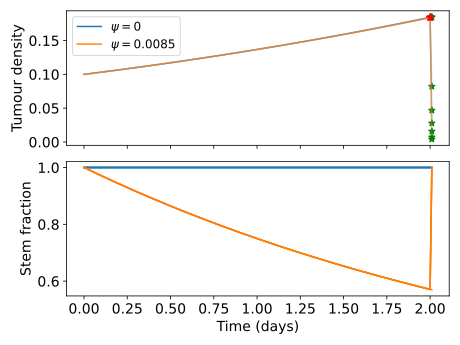
\includegraphics{images/png/simulated_RT_assay_GBM1a.png}

}

\subcaption{\label{fig-sim_RT_assay_GBM1a}}

\end{minipage}%
%
\begin{minipage}{0.50\linewidth}

\centering{

\includegraphics{images/png/simulated_dose_response_GBM1a.png}

}

\subcaption{\label{fig-sim_dose_response_GBM1a}}

\end{minipage}%
\newline
\begin{minipage}{\linewidth}

\centering{

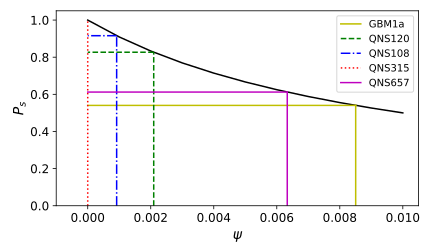
\includegraphics{images/png/psi_values_visualised.png}

}

\subcaption{\label{fig-psi_values_visualised}}

\end{minipage}%

\caption{\label{fig-days_gained_example_sim}Simulated radiotherapy
assay. (a) Initially a small number of cells were seeded (represented by
a small density of tumor cells). These were grown for 2 days under
either control or 100ng/ml BMP4. After 2 days, radiotherapy was applied
at different dosages and the number of surviving colonies were counted.
The red star indicates when RT was applied (48 hrs) and the green stars
indicate the final measured density of tumor immediately after
radiotherapy for different doses of radiation. (b) Simulated dose
response to radiotherapy after fitting \(\psi\) in the ODE model to
provide the expected fraction of GSCs given the doubling time of the
cell line. (c) Each of the cell lines has a distinct sensitivity to BMP4
denoted \(\psi\).}

\end{figure}%

\begin{longtable}[]{@{}
  >{\raggedright\arraybackslash}p{(\columnwidth - 10\tabcolsep) * \real{0.1667}}
  >{\raggedright\arraybackslash}p{(\columnwidth - 10\tabcolsep) * \real{0.1667}}
  >{\raggedright\arraybackslash}p{(\columnwidth - 10\tabcolsep) * \real{0.1667}}
  >{\raggedright\arraybackslash}p{(\columnwidth - 10\tabcolsep) * \real{0.1667}}
  >{\raggedright\arraybackslash}p{(\columnwidth - 10\tabcolsep) * \real{0.1667}}
  >{\raggedright\arraybackslash}p{(\columnwidth - 10\tabcolsep) * \real{0.1667}}@{}}
\caption{Fitted parameter values and metadata from cell lines. All cell
lines are from primary tumor. It is assumed that \(\alpha/\beta = 10\)
is fixed for all cell lines.}\label{tbl-RT-data}\tabularnewline
\toprule\noalign{}
\begin{minipage}[b]{\linewidth}\raggedright
Cell line
\end{minipage} & \begin{minipage}[b]{\linewidth}\raggedright
\(\alpha\)
\end{minipage} & \begin{minipage}[b]{\linewidth}\raggedright
F
\end{minipage} & \begin{minipage}[b]{\linewidth}\raggedright
Doubling time (hrs)
\end{minipage} & \begin{minipage}[b]{\linewidth}\raggedright
Sensitivity to BMP4 (\(\psi\))
\end{minipage} & \begin{minipage}[b]{\linewidth}\raggedright
Sex
\end{minipage} \\
\midrule\noalign{}
\endfirsthead
\toprule\noalign{}
\begin{minipage}[b]{\linewidth}\raggedright
Cell line
\end{minipage} & \begin{minipage}[b]{\linewidth}\raggedright
\(\alpha\)
\end{minipage} & \begin{minipage}[b]{\linewidth}\raggedright
F
\end{minipage} & \begin{minipage}[b]{\linewidth}\raggedright
Doubling time (hrs)
\end{minipage} & \begin{minipage}[b]{\linewidth}\raggedright
Sensitivity to BMP4 (\(\psi\))
\end{minipage} & \begin{minipage}[b]{\linewidth}\raggedright
Sex
\end{minipage} \\
\midrule\noalign{}
\endhead
\bottomrule\noalign{}
\endlastfoot
GBM1a & 0.338 & 0.571 & 54.7 & 0.00850409 & Male \\
QNS120 & 0.116 & 0.770 & 43.5 & 0.002094342 & Male \\
QNS108 & 0.151 & 0.949 & 109 & 0.000918066 & Male \\
QNS315 & 0.0841 & 1 & 63.6 & 0 & Female \\
QNS657 & 0.104 & 0.707 & 75.6 & 0.006332659 & Female \\
\end{longtable}

\subsection{Model simulations}\label{sec-model-sims}

We simulate our model for a range of parameter values to explore the
effect of BMP4 on tumor growth. Based on our fitted values of \(\psi\)
we consider a range from \([0,0.1]\), the full parameter values are
given in Table~\ref{tbl-params}. To simulate treatment we allow the
model to run until the total tumor size reaches \(0.2\), then initiate
treatment. To evaluate the effect of BMP4, we compare two treatment
arms: standard of care - resection (at the time of detection) followed
by radiotherapy 30 days later, and BMP4 - standard of care with the
addition of BMP4. To observe the effect of BMP4, we assume a fixed
concentration of AMSCs, which release BMP4 at a constant rate, from the
time of resection until the end of radiotherapy. In each case we record
the number of days until the tumor reaches a size of \(0.6\) and refer
to this as time to progression. This allows us to calculate the fold
change in time to progression to directly compare for each set of
parameters how much the BMP4 prolonged survival. The results are shown
in Figure~\ref{fig-days_gained}.

Since GSCs are less sensitive to RT than other cells, the fraction of
GSCs increases during RT; this is shown in our model in
Figure~\ref{fig-example_sims}. In particular, radiotherapy is more
effective against faster proliferating tumors (R. Rockne et al. 2010) so
this effect is particularly pronounced in these tumors. Enrichment of
GSCs during RT not only highlights that there are some resistant cells
not being targeted by radiotherapy but also since these are the most
tumorigenic cells, with a large proportion of GSCs, a recurrent tumor is
able to form rapidly (as compared to not at all if no GSCs were
present). When we simulated the addition of BMP4 (the dashed lines in
Figure~\ref{fig-example_sims}) we see that this peak in stem-cell
fraction is reduced due to the induced differentiation of GSCs. This
means that not only is the RT more effective as there are fewer
resistant GSCs but also that the tumor will take longer to recur as
there are fewer GSCs to drive regrowth. As the increase in GSC fraction
is most pronounced in faster proliferating tumors, we see that the
relative effect of BMP4 in delaying progression is also largest for
these patients.

\begin{longtable}[]{@{}
  >{\raggedright\arraybackslash}p{(\columnwidth - 8\tabcolsep) * \real{0.2000}}
  >{\raggedright\arraybackslash}p{(\columnwidth - 8\tabcolsep) * \real{0.2000}}
  >{\raggedright\arraybackslash}p{(\columnwidth - 8\tabcolsep) * \real{0.2000}}
  >{\raggedright\arraybackslash}p{(\columnwidth - 8\tabcolsep) * \real{0.2000}}
  >{\raggedright\arraybackslash}p{(\columnwidth - 8\tabcolsep) * \real{0.2000}}@{}}
\caption{Table of parameter values used. When the value is fixed its
value is given, if it is sampled from a distribution then the
distribution is given.}\label{tbl-params}\tabularnewline
\toprule\noalign{}
\begin{minipage}[b]{\linewidth}\raggedright
Parameter
\end{minipage} & \begin{minipage}[b]{\linewidth}\raggedright
Meaning
\end{minipage} & \begin{minipage}[b]{\linewidth}\raggedright
Value / distribution
\end{minipage} & \begin{minipage}[b]{\linewidth}\raggedright
Units
\end{minipage} & \begin{minipage}[b]{\linewidth}\raggedright
Reference
\end{minipage} \\
\midrule\noalign{}
\endfirsthead
\toprule\noalign{}
\begin{minipage}[b]{\linewidth}\raggedright
Parameter
\end{minipage} & \begin{minipage}[b]{\linewidth}\raggedright
Meaning
\end{minipage} & \begin{minipage}[b]{\linewidth}\raggedright
Value / distribution
\end{minipage} & \begin{minipage}[b]{\linewidth}\raggedright
Units
\end{minipage} & \begin{minipage}[b]{\linewidth}\raggedright
Reference
\end{minipage} \\
\midrule\noalign{}
\endhead
\bottomrule\noalign{}
\endlastfoot
\(\delta_s\) & death rate of GSCs & 0.001 & 1 / year & Estimated \\
\(\delta_i\) & death rate of PCs & 0.01 & 1 / year & Estimated \\
\(\delta_n\) & death rate of TCs & 0.1 & 1 / year & Estimated \\
\(\delta_m\) & death rate of AMSCs & 0.5 & 1 / year & (Li et al.
2014) \\
\(\delta_B\) & Decay rate of BMP4 & 0.5 & 1 / year & (Li et al. 2014) \\
\(u_B\) & Uptake rate of BMP4 & 0.5 & 1 / year & Estimated \\
\(C\) & Release rate of BMP4 from AMSCs & 0.5 & 1 / year & Estimated \\
n & Number of division of PCs & 10 & - & (Gao et al. 2013) \\
\(m_i\) & Proliferation rate of PCs & \(\text{log-N}(2.75,0.51)\) & 1 /
year & (Yang et al. 2019) \\
\(m_s\) & Proliferation rate of GSCs & \(0.0345 m_i\) & 1 / year &
Estimated \\
\(\alpha\) & Radiosensitivity & \(0.05 m_i\) & 1 / Gy & (R. Rockne et
al. 2010) \\
\end{longtable}

\begin{figure}

\begin{minipage}{0.50\linewidth}

\centering{

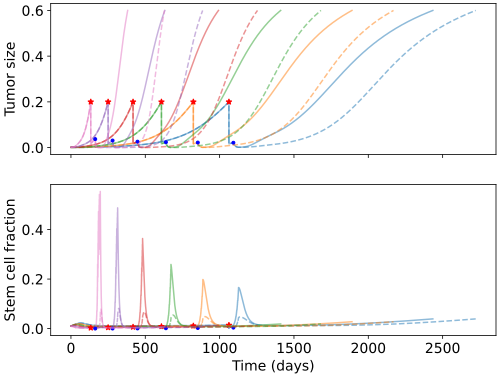
\includegraphics{images/png/example_sims.png}

}

\subcaption{\label{fig-example_sims}}

\end{minipage}%
%
\begin{minipage}{0.50\linewidth}

\centering{

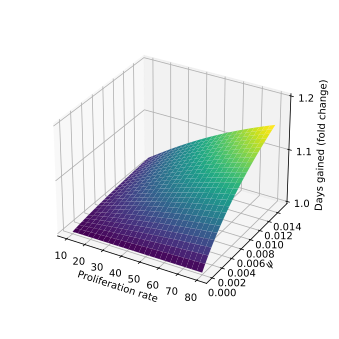
\includegraphics{images/png/days_gained.png}

}

\subcaption{\label{fig-days_gained}}

\end{minipage}%

\caption{\label{fig-effect_BMP4}Effect of BMP4 on tumor progression. (a)
Example model simulations showing the total tumor density and fraction
of GSCs. Red stars indicate when the tumor was detected at \(N=0.2\) and
the blue dot represents the start of radiotherapy (30 days later).
Simulated standard of care (resection and radiotherapy) is plotted in
solid lines and BMP4-AMSCs is in the dashed lines. During radiotherapy
the fraction of GSCs is greatly increased as they are less sensitive
than the non-GSCs. When BMP4 is added this enrichment in GSCs is
reduced, delaying time for tumor regrowth. (b) Days gained surface. As
we increase both the sensitivity to BMP4 (\(\psi\)) and the
proliferation rate the fold change in time to progression increases.}

\end{figure}%

\subsection{Virtual clinical trial
pipeline}\label{sec-virtual-trial-pipeline}

Firstly we simulate a large cohort of virtual patients with fix
sensitivity to BMP4 based on the parameters identified in
Section~\ref{sec-simulating-RT-experiments}. We compare our simulated
BMP4 patients to virtual controls to show that BMP4 can delay tumor
growth. We then develop a pipeline for simulating early-phase 2 clinical
trials and calculating the probability of observing a successful trial.

\subsubsection{Uncertainty in tumor detection and
death}\label{sec-unce-death-detect}

We assume that both detection of the tumor and death depend on tumor
size in a random fashion for each virtual patient. Detection (death) is
more likely the bigger a tumor is, but two tumors of equal size in two
patients do not necessarily lead to detection (death) at the same times.
Thus, we assume that the times of tumor detection and death, represented
by the random variables \(T_{\text{detect}}\) and \(T_{\text{death}}\),
depend on total tumor density \(N(t)\) according to the hazard function

\begin{equation}\phantomsection\label{eq-detect_death_hazard}{
  P(T_d \in [t,t+\Delta t) | T_d>t) = \lambda_d (N(t)) \Delta t + o(\Delta t), \quad d \in \{\text{detect},\text{death}\},
}\end{equation}

where

\begin{equation}\phantomsection\label{eq-lambda_N}{
  \lambda_d (N) = \frac{\lambda_{d,\text{max}}}{1 + e^{-m_d(N - N_d)}}.
}\end{equation}

Here, \(\lambda_d(N)\) is a shifted logistic function;
\(\lambda_{d,\text{max}}\) is the maximum rate of detection that we take
to be 1, \(m_d\) describes the steepness of the logistic function, which
we set to be 100 in the detection case and 20 in the death case. The
constant \(N_d\) is a threshold parameter at which the probability rate
of detection or death is half-maximal (each of these for
\(d\in\{\text{detect},\text{death}\}\)), we set this to be 0.2 and 0.7
in the detection and death cases respectively. \(\Delta t\) is the
timestep on which the model is solved numerically. This is similar to
the approach of (Bartoszyński et al. 2001; Plevritis et al. 2006), apart
from our choice of nonlinear dependence on tumor size. The shifted
logistic function acts as a switch mechanism, meaning once \(N > N_d\)
the rate of detection or death rapidly increases towards its maximum.
Figure~\ref{fig-detect_death} shows the form of these functions with the
parameters used in the virtual trials that follow.

\subsubsection{Simulated control virtual patient
population}\label{sec-simulation-controls}

To construct a group of control patients, we sample proliferation rates
from a distribution consistent with measured proliferation rates of
around 300 patients (Yang et al. 2019), from this distribution we sample
200 patients. We then simulate these patients undergoing resection and
radiotherapy (standard of care); to consider the effect of BMP4 on
survival we assume a constant concentration of 100ng/ml is maintained
from detection until the end of radiotherapy and we consider two
different sensitivities \(\psi = 0.0021\) and \(\psi = 0.0085\), these
values correspond with the cell lines QNS120 and GBM1a from
Table~\ref{tbl-RT-data}. The results are shown in
Figure~\ref{fig-simulated-controls}. We see that BMP4 improves simulated
survival times and that as the sensitivity to BMP4 is increased the
response is more pronounced.

\begin{figure}

\begin{minipage}{0.50\linewidth}

\centering{

\includegraphics{images/png/detect_death.png}

}

\subcaption{\label{fig-detect_death}}

\end{minipage}%
%
\begin{minipage}{0.50\linewidth}

\centering{

\includegraphics{images/png/hist_data.png}

}

\subcaption{\label{fig-hist_data}}

\end{minipage}%
\newline
\begin{minipage}{0.50\linewidth}

\centering{

\includegraphics{images/png/sim_control_example_sims.png}

}

\subcaption{\label{fig-example_sims_control}}

\end{minipage}%
%
\begin{minipage}{0.50\linewidth}

\centering{

\includegraphics{images/png/simulate_control_KM.png}

}

\subcaption{\label{fig-simulated_control_KM}}

\end{minipage}%

\caption{\label{fig-simulated-controls}Simulated virtual control
patients. (a) Tumor detection and death are considered random events
which increase in probability as tumor size increases. (b) Histogram of
proliferation rates from (Yang et al. 2019), red line shows fitted log
normal distribution (c) Example model simulation trajectories showing
overall tumor density and fraction of stem cells. The red stars indicate
when the tumor was detected and the blue dots when radiotherapy was
started. (d) Comparison of survival times for simulated control patients
(resection and radiotherapy) with BMP4 treatment, for two different
sensitivities to BMP4.}

\end{figure}%

\subsubsection{Simulated phase 2 trial}\label{sec-phase-2-trial}

In practice a phase 2 trial will have only a small number of patients
(typically around 20-40) and the population will be heterogeneous with
respect to sensitivity to BMP4. We develop a virtual trial pipeline to
consider the chance of observing a successful trial for different
virtual populations. We have previously observed that proliferation rate
can impact the efficacy of BMP4 treatment
(Figure~\ref{fig-days_gained}). Therefore, we consider 3 stratifications
of the population based on proliferation rate. We construct these by
sampling twice as many virtual patients as we need for each trial (80)
and then splitting them into either the top 50\% fastest proliferators,
the middle 50\%, or the slowest 50\%, so that each group has 40 virtual
patients. We then split them via a stratified random split, so that both
groups have similar distributions of proliferation rates, into control
and treatment arms (20 in each), with parameters drawn from
Table~\ref{tbl-params} and \(\psi\) from a truncated normal
distribution. This assumes knowledge of growth rates for patients
enrolled in the trial, which is straightforward for our simulated
virtual patients. For each group (fast, medium, slow) we perform 20
virtual trials, each one comprising a distinct set of 40 patients,
giving us an idea of the chance of observing a successful trial.

We assume a distribution of sensitivities drawn from a truncated normal
distribution with mean sensitivity \(\psi_\text{mean} = 0.0085\), so
that, according to our model fits this would be a population that has
been identified as highly sensitive to BMP4. For this cohort of virtual
patients we consider a possible delivery schedule of BMP4-AMSCs which we
shall term `single-hit', this consists of a single dose of AMSCs-BMP4 at
the time of resection. This is a promising and practical option for
BMP4-AMSCs delivery as they can be implanted directly into the tumor at
the time of resection and means the patient is receiving some treatment
in the time between resection and radiotherapy, when typically they
receive none during this time. For this cohort of virtual patients, we
implement a series of different concentrations of AMSCs-BMP4; in
Figure~\ref{fig-Identical_mid_KM} we show average BMP4 concentration in
ng/ml, to compare this to the radiotherapy assay in
Section~\ref{sec-simulating-RT-experiments}. An average concentration of
8ng/ml corresponds to a peak of 100ng/ml at the time of resection, the
same concentration maintained for two days in the assay. We see that,
for peak concentrations of BMP4 similar to that in the \emph{in vitro}
assay, no trials show statistically significant differences in survival
curves (log-rank test, \(p>0.05\)). Indeed, according to these results a
considerably higher total dose of BMP4 is required in order to see
consistently successful trials (defined as rejecting the null hypothesis
of identical survival curves between control and treatment arms). This
may be because of the relatively rapid decay of AMSCs and BMP4; if ASMCs
are delivered at the time of resection very few remain and BMP4
concentrations are low by the time RT begins.

The results plotted in Figure~\ref{fig-Identical_mid_KM} are for the
group of fast proliferators only as this was the only group which saw a
significant response to BMP4 therapy.
Figure~\ref{fig-phase2_trial_summary} shows a summary of the results for
all the proliferation groups. This highlights the importance of
considering other patient specific parameters when selecting potential
patients for clinical trial.

\begin{figure}

\begin{minipage}{0.50\linewidth}

\centering{

\includegraphics{images/png/virtual_trial_BMP4_200_rho_case_5.png}

}

\subcaption{\label{fig-example2}}

\end{minipage}%
%
\begin{minipage}{0.50\linewidth}

\centering{

\includegraphics{images/png/virtual_trial_BMP4_500_rho_case_5.png}

}

\subcaption{\label{fig-example3}}

\end{minipage}%
\newline
\begin{minipage}{0.50\linewidth}

\centering{

\includegraphics{images/png/virtual_trial_BMP4_1000_rho_case_5.png}

}

\subcaption{\label{fig-ex-4}}

\end{minipage}%
%
\begin{minipage}{0.50\linewidth}

\centering{

\includegraphics{images/png/prob_succ_strat.png}

}

\subcaption{\label{fig-phase2_trial_summary}}

\end{minipage}%

\caption{\label{fig-Identical_mid_KM}Survival curves for 20 simulated
virtual trials for the fast proliferating stratification shaded by
success (if BMP4 treatment arm is significantly different to the control
arm) for four different concentrations of BMP4. (a) As expected, when
BMP4 is low the control and treatment arms are similar in all 20 trials.
(b) As BMP4 concentration increases, the fraction of successful trials
increases. (c) For sufficiently high BMP4 (and hence a sufficiently
strong treatment effect), almost all trials are successful. (d) Summary
of the successful trial from phase 2. Orange, green and blue represent
fast, medium and slow proliferation, respectively.}

\end{figure}%

\subsubsection{Different delivery schedules for
BMP4}\label{different-delivery-schedules-for-bmp4}

The high concentrations of BMP4 required in a single-hit approach
identified in Section~\ref{sec-phase-2-trial} motivates us to look at
alternative dosing strategies, where similar or greater benefit may be
observed for less average dose of BMP4. As the AMSCs only last for
around 2 weeks (and BMP4 slightly less) only a small concentration is
left by the time radiotherapy occurs in the single-hit approach. Since
BMP4 increases the radiosensitivity of the tumor and reduces the
enrichment of GSCs when radiotherapy occurs, delivering it in
combination with radiotherapy may provide significantly improved
responses even when a similar total dose of BMP4 is considered.
Therefore, we consider 3 alternative treatment schedules: i) a single
dose immediately before radiotherapy, ii) a continuous dose from
resection until the end of RT and iii) periodic doses in combination
with radiotherapy. These schedules are shown in
Figure~\ref{fig-delivery_schedule}. In all cases, the same total dose of
BMP4 (this corresponds to the same area under the curve in
Figure~\ref{fig-delivery_schedule}) will be administered so the
comparison is fair between delivery schedules.

We use the same virtual trial pipeline outlined previously in
Section~\ref{sec-virtual-trial-pipeline}, applied to these three
alternative dosing strategies. A summary of the results for the fast
proliferating group is plotted in
Figure~\ref{fig-delivery_schedule_frac_succ}. We see that the continuous
delivery schedule is the most effective, with the highest number of
successful trials with an average BMP4 concentration of around 10ng/ml
required for almost all trials to be successful. This is closely
followed by the periodic schedule. The shifted single dose appears to be
largely similar in efficacy as the single dose at resection. These show
that longer term exposure of BMP4 greatly increases its efficacy. This
highlights the importance of designing the delivery schedule of BMP4 to
maximise the effect of the treatment, and in future could be optimised
on a patient-specific level.

\begin{figure}

\begin{minipage}{0.50\linewidth}

\centering{

\includegraphics{images/png/BMP4_delivery_schedule.png}

}

\subcaption{\label{fig-delivery_schedule}}

\end{minipage}%
%
\begin{minipage}{0.50\linewidth}

\centering{

\includegraphics{images/png/diff_schedules_frac_succ.png}

}

\subcaption{\label{fig-delivery_schedule_frac_succ}}

\end{minipage}%

\caption{\label{fig-delivery_schedule_frac_succ_overall}Alternative
delivery schedules have improved response to BPM4 for same total dose.
(a) Different delivery schedules for BMP4. Here time 0 represents the
time of detection and radiotherapy occurs 30 days after detection. (b)
Summary of fraction of successful trails for different delivery
schedules.}

\end{figure}%

\section{Discussion}\label{sec-discussion}

In this study, we have developed a comprehensive mathematical model to
simulate GSC-driven tumor growth, specifically focusing on the impact of
BMP4 treatment. By parameterizing our model using experimental data from
five distinct glioma stem cell lines exposed to BMP4, we were able to
qualitatively estimate the sensitivity of these cell lines to BMP4. This
approach provides valuable insights into the potential variability in
treatment response among different glioma cell populations.

A key limitation of our model lies in the inherent assumptions necessary
for reducing the complex biology of glioblastoma/glioma to a system of
ordinary differential equations (ODEs). While our model successfully
encapsulates many aspects of tumor dynamics, it does not explicitly
account for the spatial heterogeneity of glioblastoma. Future work could
expand this model to incorporate spatial considerations, to better
capture the intricate microenvironment and its influence on tumor
behaviour. That said, we hope that capturing the essence of the proposed
BMP4 treatment in the current model has highlighted key mechanisms by
which impact on tumor growth may or may not be seen in the clinic.

Moreover, our study primarily concentrated on the impact of BMP4-induced
differentiation on radiosensitivity, leaving the direct effects of BMP4
on proliferation rates as an area for further exploration. Understanding
how BMP4 modulates proliferation, in addition to differentiation, could
provide a more comprehensive picture of its therapeutic potential and
guide the development of more effective treatment strategies.

Importantly, we have also demonstrated a virtual clinical trial pipeline
to evaluate the potential of BMP4-AMSCs treatment for patients with GBM.
Our simulations revealed that a significant amount of BMP4 would be
required to achieve successful outcomes in a substantial proportion of
patients. This finding underscores the importance of optimizing BMP4
dosage and delivery methods for future clinical applications.
Additionally, our results suggest that patient stratification based on
proliferation rates could enhance the likelihood of treatment success.
By selecting patients with higher proliferation rates, we could
potentially increase the observed efficacy of BMP4 in combination with
radiotherapy.

Furthermore, we explored various BMP4 delivery schedules and identified
that alternative strategies could enhance the therapeutic synergy
between BMP4 and radiotherapy. These findings indicate that the timing
and duration of BMP4 administration, in particular in relation to the
timing of radiotherapy, can be crucial factors that could be optimized
to improve clinical outcomes. We have shown that prolonged exposure to
BMP4 greatly increased it efficacy when compared to a `single-hit'
approach. Future studies could expand on this by investigating different
delivery modalities and schedules, potentially in combination with other
therapies, to maximize the therapeutic benefit of BMP4.

In conclusion, our work provides a robust framework for virtual clinical
trials, offering valuable predictions that can guide the clinical
translation of BMP4-based therapies for GBM. By highlighting the need
for high BMP4 levels, patient stratification, and optimized delivery
strategies, we have laid the groundwork for future studies that can
further refine and validate these approaches in a clinical context.

\section*{References}\label{references}
\addcontentsline{toc}{section}{References}

\phantomsection\label{refs}
\begin{CSLReferences}{1}{0}
\bibitem[\citeproctext]{ref-al-hajj2003}
Al-Hajj, Muhammad, Max S. Wicha, Adalberto Benito-Hernandez, Sean J.
Morrison, and Michael F. Clarke. 2003. {``Prospective Identification of
Tumorigenic Breast Cancer Cells.''} \emph{Proceedings of the National
Academy of Sciences} 100 (7): 3983--88.
\url{https://doi.org/10.1073/pnas.0530291100}.

\bibitem[\citeproctext]{ref-bachman2013}
Bachman, Jeff W. N., and Thomas Hillen. 2013. {``Mathematical
Optimization of the Combination of Radiation and Differentiation
Therapies for Cancer.''} \emph{Frontiers in Oncology} 3.
\url{https://doi.org/10.3389/fonc.2013.00052}.

\bibitem[\citeproctext]{ref-bagley2022}
Bagley, Stephen J., Shawn Kothari, Rifaquat Rahman, Eudocia Q. Lee,
Gavin P. Dunn, Evanthia Galanis, Susan M. Chang, et al. 2022.
{``Glioblastoma Clinical Trials: Current Landscape and Opportunities for
Improvement.''} \emph{Clinical Cancer Research} 28 (4): 594--602.
\url{https://doi.org/10.1158/1078-0432.CCR-21-2750}.

\bibitem[\citeproctext]{ref-bao2006}
Bao, Shideng, Qiulian Wu, Roger E. McLendon, Yueling Hao, Qing Shi,
Anita B. Hjelmeland, Mark W. Dewhirst, Darell D. Bigner, and Jeremy N.
Rich. 2006. {``Glioma Stem Cells Promote Radioresistance by Preferential
Activation of the DNA Damage Response.''} \emph{Nature} 444 (7120):
756--60. \url{https://doi.org/10.1038/nature05236}.

\bibitem[\citeproctext]{ref-bartoszynski2001}
Bartoszyński, Robert, Lutz Edler, Leonid Hanin, Annette Kopp-Schneider,
Lyudmila Pavlova, Alexander Tsodikov, Alexander Zorin, and Andrej Yu.
Yakovlev. 2001. {``Modeling Cancer Detection: Tumor Size as a Source of
Information on Unobservable Stages of Carcinogenesis.''}
\emph{Mathematical Biosciences} 171 (2): 113--42.
\url{https://doi.org/10.1016/s0025-5564(01)00058-x}.

\bibitem[\citeproctext]{ref-bonnet1997}
Bonnet, Dominique, and John E. Dick. 1997. {``Human Acute Myeloid
Leukemia Is Organized as a Hierarchy That Originates from a Primitive
Hematopoietic Cell.''} \emph{Nature Medicine} 3 (7): 730--37.
\url{https://doi.org/10.1038/nm0797-730}.

\bibitem[\citeproctext]{ref-cardinal2022}
Cardinal, Olivia, Chloé Burlot, Yangxin Fu, Powel Crosley, Mary Hitt,
Morgan Craig, and Adrianne L. Jenner. 2022. {``Establishing Combination
PAC{-}1 and TRAIL Regimens for Treating Ovarian Cancer Based on
Patient{-}Specific Pharmacokinetic Profiles Using {\emph{in Silico}}
Clinical Trials.''} \emph{Computational and Systems Oncology} 2 (2).
\url{https://doi.org/10.1002/cso2.1035}.

\bibitem[\citeproctext]{ref-caruxe9n2016}
Carén, Helena, Stephan Beck, and Steven M. Pollard. 2016.
{``Differentiation Therapy for Glioblastoma {\textendash} Too Many
Obstacles?''} \emph{Molecular \& Cellular Oncology} 3 (2): e1124174.
\url{https://doi.org/10.1080/23723556.2015.1124174}.

\bibitem[\citeproctext]{ref-chaichana2014}
Chaichana, Kaisorn L., Eibar Ernesto Cabrera-Aldana, Ignacio
Jusue-Torres, Olindi Wijesekera, Alessandro Olivi, Maryam Rahman, and
Alfredo Quinones-Hinojosa. 2014. {``When Gross Total Resection of a
Glioblastoma Is Possible, How Much Resection Should Be Achieved?''}
\emph{World Neurosurgery} 82 (1-2): e257--65.
\url{https://doi.org/10.1016/j.wneu.2014.01.019}.

\bibitem[\citeproctext]{ref-cloughesy2020}
Cloughesy, Timothy F., Kevin Petrecca, Tobias Walbert, Nicholas
Butowski, Michael Salacz, James Perry, Denise Damek, et al. 2020.
{``Effect of Vocimagene Amiretrorepvec in Combination With Flucytosine
Vs Standard of Care on Survival Following Tumor Resection in Patients
With Recurrent High-Grade Glioma: A Randomized Clinical Trial.''}
\emph{JAMA Oncology} 6 (12): 1939.
\url{https://doi.org/10.1001/jamaoncol.2020.3161}.

\bibitem[\citeproctext]{ref-craig2023}
Craig, Morgan, Jana L. Gevertz, Irina Kareva, and Kathleen P. Wilkie.
2023. {``A Practical Guide for the Generation of Model-Based Virtual
Clinical Trials.''} \emph{Frontiers in Systems Biology} 3 (June).
\url{https://doi.org/10.3389/fsysb.2023.1174647}.

\bibitem[\citeproctext]{ref-dethuxe92018}
De Thé, Hugues. 2018. {``Differentiation Therapy Revisited.''}
\emph{Nature Reviews Cancer} 18 (2): 117--27.
\url{https://doi.org/10.1038/nrc.2017.103}.

\bibitem[\citeproctext]{ref-dingli2006}
Dingli, David, and Franziska Michor. 2006. {``Successful Therapy Must
Eradicate Cancer Stem Cells.''} \emph{STEM CELLS} 24 (12): 2603--10.
\url{https://doi.org/10.1634/stemcells.2006-0136}.

\bibitem[\citeproctext]{ref-dirks2006}
Dirks, Peter B. 2006. {``Stem Cells and Brain Tumours.''} \emph{Nature}
444 (7120): 687--88. \url{https://doi.org/10.1038/444687a}.

\bibitem[\citeproctext]{ref-doucette2011}
Doucette, Tiffany, Ganesh Rao, Yuhui Yang, Joy Gumin, Naoki Shinojima,
B. Nebiyou Bekele, Wei Qiao, Wei Zhang, and Frederick F. Lang. 2011.
{``Mesenchymal Stem Cells Display Tumor-Specific Tropism in an
RCAS/Ntv-a Glioma Model.''} \emph{Neoplasia} 13 (8): 716--25.
\url{https://doi.org/10.1593/neo.101680}.

\bibitem[\citeproctext]{ref-dowden2019}
Dowden, Helen, and Jamie Munro. 2019. {``Trends in Clinical Success
Rates and Therapeutic Focus.''} \emph{Nature Reviews Drug Discovery} 18
(7): 495--96. \url{https://doi.org/10.1038/d41573-019-00074-z}.

\bibitem[\citeproctext]{ref-enderling2009}
Enderling, H, L Hlatky, and P Hahnfeldt. 2009. {``Migration Rules:
Tumours Are Conglomerates of Self-Metastases.''} \emph{British Journal
of Cancer} 100 (12): 1917--25.
\url{https://doi.org/10.1038/sj.bjc.6605071}.

\bibitem[\citeproctext]{ref-farias}
Farias, Virgina, Vinitha Rani, Natanael Zacro, Mieu Brooks, Naveen
Nagaiah, Henry Ruiz-Garcia, Rachel Sarabia-Estrada, et al. n.d.
{``BMP4-Secreting MSCs Derived from Human Adipose Tissue Radiosensitize
Glioblastoma Stem Cells via Downregulation of OLIG2 Signaling
Pathway.''} \emph{In Preparation}.

\bibitem[\citeproctext]{ref-galli2004}
Galli, Rossella, Elena Binda, Ugo Orfanelli, Barbara Cipelletti, Angela
Gritti, Simona De Vitis, Roberta Fiocco, Chiara Foroni, Francesco
Dimeco, and Angelo Vescovi. 2004. {``Isolation and Characterization of
Tumorigenic, Stem-Like Neural Precursors from Human Glioblastoma.''}
\emph{Cancer Research} 64 (19): 7011--21.
\url{https://doi.org/10.1158/0008-5472.CAN-04-1364}.

\bibitem[\citeproctext]{ref-gao2013}
Gao, Xuefeng, J. Tyson McDonald, Lynn Hlatky, and Heiko Enderling. 2013.
{``Acute and Fractionated Irradiation Differentially Modulate Glioma
Stem Cell Division Kinetics.''} \emph{Cancer Research} 73 (5): 1481--90.
\url{https://doi.org/10.1158/0008-5472.CAN-12-3429}.

\bibitem[\citeproctext]{ref-griffin2006}
Griffin, Robert J. 2006. {``Radiobiology for the Radiologist, 6th
Edition.''} \emph{International Journal of Radiation
Oncology*Biology*Physics} 66 (2): 627.
\url{https://doi.org/10.1016/j.ijrobp.2006.06.027}.

\bibitem[\citeproctext]{ref-guerrero-cuxe1zares2014}
Guerrero-Cázares, Hugo, Stephany Y. Tzeng, Noah P. Young, Ameer O.
Abutaleb, Alfredo Quiñones-Hinojosa, and Jordan J. Green. 2014.
{``Biodegradable Polymeric Nanoparticles Show High Efficacy and
Specificity at DNA Delivery to Human Glioblastoma {\emph{in Vitro}} and
{\emph{in Vivo}}.''} \emph{ACS Nano} 8 (5): 5141--53.
\url{https://doi.org/10.1021/nn501197v}.

\bibitem[\citeproctext]{ref-hemmati2003}
Hemmati, Houman D., Ichiro Nakano, Jorge A. Lazareff, Michael
Masterman-Smith, Daniel H. Geschwind, Marianne Bronner-Fraser, and
Harley I. Kornblum. 2003. {``Cancerous Stem Cells Can Arise from
Pediatric Brain Tumors.''} \emph{Proceedings of the National Academy of
Sciences} 100 (25): 15178--83.
\url{https://doi.org/10.1073/pnas.2036535100}.

\bibitem[\citeproctext]{ref-ignatova2002}
Ignatova, Tatyana N., Valery G. Kukekov, Eric D. Laywell, Oleg N.
Suslov, Frank D. Vrionis, and Dennis A. Steindler. 2002. {``Human
Cortical Glial Tumors Contain Neural Stem{-}Like Cells Expressing
Astroglial and Neuronal Markers in Vitro.''} \emph{Glia} 39 (3):
193--206. \url{https://doi.org/10.1002/glia.10094}.

\bibitem[\citeproctext]{ref-kim2016}
Kim, Eunjung, Vito W. Rebecca, Keiran S. M. Smalley, and Alexander R. A.
Anderson. 2016. {``Phase i Trials in Melanoma: A Framework to Translate
Preclinical Findings to the Clinic.''} \emph{European Journal of Cancer}
67 (November): 213--22.
\url{https://doi.org/10.1016/j.ejca.2016.07.024}.

\bibitem[\citeproctext]{ref-kim2020}
Kim, Jayoung, Sujan K. Mondal, Stephany Y. Tzeng, Yuan Rui, Rawan
Al-kharboosh, Kristen K. Kozielski, Adip G. Bhargav, Cesar A. Garcia,
Alfredo Quiñones-Hinojosa, and Jordan J. Green. 2020. {``Poly(ethylene
Glycol){\textendash}Poly(beta-Amino Ester)-Based Nanoparticles for
Suicide Gene Therapy Enhance Brain Penetration and Extend Survival in a
Preclinical Human Glioblastoma Orthotopic Xenograft Model.''} \emph{ACS
Biomaterials Science \& Engineering} 6 (5): 2943--55.
\url{https://doi.org/10.1021/acsbiomaterials.0c00116}.

\bibitem[\citeproctext]{ref-lapidot1994}
Lapidot, Tsvee, Christian Sirard, Josef Vormoor, Barbara Murdoch, Trang
Hoang, Julio Caceres-Cortes, Mark Minden, Bruce Paterson, Michael A.
Caligiuri, and John E. Dick. 1994. {``A Cell Initiating Human Acute
Myeloid Leukaemia After Transplantation into SCID Mice.''} \emph{Nature}
367 (6464): 645--48. \url{https://doi.org/10.1038/367645a0}.

\bibitem[\citeproctext]{ref-lee2016}
Lee, Yeri, Jin-Ku Lee, Sun Hee Ahn, Jeongwu Lee, and Do-Hyun Nam. 2016.
{``WNT Signaling in Glioblastoma and Therapeutic Opportunities.''}
\emph{Laboratory Investigation} 96 (2): 137--50.
\url{https://doi.org/10.1038/labinvest.2015.140}.

\bibitem[\citeproctext]{ref-li2014}
Li, Qian, Olindi Wijesekera, Sussan J. Salas, Joanna Y. Wang, Mingxin
Zhu, Colette Aprhys, Kaisorn L. Chaichana, et al. 2014. {``Mesenchymal
Stem Cells from Human Fat Engineered to Secrete BMP4 Are Nononcogenic,
Suppress Brain Cancer, and Prolong Survival.''} \emph{Clinical Cancer
Research} 20 (9): 2375--87.
\url{https://doi.org/10.1158/1078-0432.CCR-13-1415}.

\bibitem[\citeproctext]{ref-ma2018}
Ma, Qianquan, Wenyong Long, Changsheng Xing, Junjun Chu, Mei Luo, Helen
Y. Wang, Qing Liu, and Rong-Fu Wang. 2018. {``Cancer Stem Cells and
Immunosuppressive Microenvironment in Glioma.''} \emph{Frontiers in
Immunology} 9 (December): 2924.
\url{https://doi.org/10.3389/fimmu.2018.02924}.

\bibitem[\citeproctext]{ref-mangraviti2016}
Mangraviti, Antonella, Stephany Y. Tzeng, David Gullotti, Kristen L.
Kozielski, Jennifer E. Kim, Michael Seng, Sara Abbadi, et al. 2016.
{``Non-Virally Engineered Human Adipose Mesenchymal Stem Cells Produce
BMP4, Target Brain Tumors, and Extend Survival.''} \emph{Biomaterials}
100 (September): 53--66.
\url{https://doi.org/10.1016/j.biomaterials.2016.05.025}.

\bibitem[\citeproctext]{ref-mcmahon2018}
McMahon, Stephen Joseph. 2018. {``The Linear Quadratic Model: Usage,
Interpretation and Challenges.''} \emph{Physics in Medicine \& Biology}
64 (1): 01TR01. \url{https://doi.org/10.1088/1361-6560/aaf26a}.

\bibitem[\citeproctext]{ref-narita2019}
Narita, Yoshitaka, Yoshiki Arakawa, Fumiyuki Yamasaki, Ryo Nishikawa,
Tomokazu Aoki, Masayuki Kanamori, Motoo Nagane, et al. 2019. {``A
Randomized, Double-Blind, Phase III Trial of Personalized Peptide
Vaccination for Recurrent Glioblastoma.''} \emph{Neuro-Oncology} 21 (3):
348--59. \url{https://doi.org/10.1093/neuonc/noy200}.

\bibitem[\citeproctext]{ref-nayak2020}
Nayak, Sonali, Ashorne Mahenthiran, Yongyong Yang, Mark McClendon,
Barbara Mania-Farnell, Charles David James, John A. Kessler, et al.
2020. {``Bone Morphogenetic Protein 4 Targeting Glioma Stem-Like Cells
for Malignant Glioma Treatment: Latest Advances and Implications for
Clinical Application.''} \emph{Cancers} 12 (2): 516.
\url{https://doi.org/10.3390/cancers12020516}.

\bibitem[\citeproctext]{ref-orourke2009}
O'Rourke, S. F. C., H. McAneney, and T. Hillen. 2009. {``Linear
Quadratic and Tumour Control Probability Modelling in External Beam
Radiotherapy.''} \emph{Journal of Mathematical Biology} 58 (4-5):
799--817. \url{https://doi.org/10.1007/s00285-008-0222-y}.

\bibitem[\citeproctext]{ref-ostrom2019}
Ostrom, Quinn T, Gino Cioffi, Haley Gittleman, Nirav Patil, Kristin
Waite, Carol Kruchko, and Jill S Barnholtz-Sloan. 2019. {``CBTRUS
Statistical Report: Primary Brain and Other Central Nervous System
Tumors Diagnosed in the United States in 2012{\textendash}2016.''}
\emph{Neuro-Oncology} 21 (Supplement{\_}5): v1--100.
\url{https://doi.org/10.1093/neuonc/noz150}.

\bibitem[\citeproctext]{ref-pendleton2013}
Pendleton, Courtney, Qian Li, David A. Chesler, Kristy Yuan, Hugo
Guerrero-Cazares, and Alfredo Quinones-Hinojosa. 2013. {``Mesenchymal
Stem Cells Derived from Adipose Tissue Vs Bone Marrow: In Vitro
Comparison of Their Tropism Towards Gliomas.''} Edited by Joseph
Najbauer. \emph{PLoS ONE} 8 (3): e58198.
\url{https://doi.org/10.1371/journal.pone.0058198}.

\bibitem[\citeproctext]{ref-piccirillo2006}
Piccirillo, S. G. M., B. A. Reynolds, N. Zanetti, G. Lamorte, E. Binda,
G. Broggi, H. Brem, A. Olivi, F. Dimeco, and A. L. Vescovi. 2006.
{``Bone Morphogenetic Proteins Inhibit the Tumorigenic Potential of
Human Brain Tumour-Initiating Cells.''} \emph{Nature} 444 (7120):
761--65. \url{https://doi.org/10.1038/nature05349}.

\bibitem[\citeproctext]{ref-plevritis2006}
Plevritis, Sylvia K., Peter Salzman, Bronislava M. Sigal, and Peter W.
Glynn. 2006. {``A Natural History Model of Stage Progression Applied to
Breast Cancer.''} \emph{Statistics in Medicine} 26 (3): 581--95.
\url{https://doi.org/10.1002/sim.2550}.

\bibitem[\citeproctext]{ref-potten1981}
Potten, C. S. 1981. {``The Cell Kinetic Mechanism for Radiation-Induced
Cellular Depletion of Epithelial Tissue Based on Hierarchical
Differences in Radiosensitivity.''} \emph{International Journal of
Radiation Biology and Related Studies in Physics, Chemistry and
Medicine} 40 (2): 217--25.
\url{https://doi.org/10.1080/09553008114551101}.

\bibitem[\citeproctext]{ref-reardon2020}
Reardon, David A., Alba A. Brandes, Antonio Omuro, Paul Mulholland,
Michael Lim, Antje Wick, Joachim Baehring, et al. 2020. {``Effect of
Nivolumab Vs Bevacizumab in Patients With Recurrent Glioblastoma: The
CheckMate 143 Phase 3 Randomized Clinical Trial.''} \emph{JAMA Oncology}
6 (7): 1003. \url{https://doi.org/10.1001/jamaoncol.2020.1024}.

\bibitem[\citeproctext]{ref-ricci-vitiani2007}
Ricci-Vitiani, Lucia, Dario G. Lombardi, Emanuela Pilozzi, Mauro
Biffoni, Matilde Todaro, Cesare Peschle, and Ruggero De Maria. 2007.
{``Identification and Expansion of Human Colon-Cancer-Initiating
Cells.''} \emph{Nature} 445 (7123): 111--15.
\url{https://doi.org/10.1038/nature05384}.

\bibitem[\citeproctext]{ref-rich2007}
Rich, Jeremy N. 2007. {``Cancer Stem Cells in Radiation Resistance.''}
\emph{Cancer Research} 67 (19): 8980--84.
\url{https://doi.org/10.1158/0008-5472.CAN-07-0895}.

\bibitem[\citeproctext]{ref-rockne2009}
Rockne, R., E. C. Alvord, J. K. Rockhill, and K. R. Swanson. 2009. {``A
Mathematical Model for Brain Tumor Response to Radiation Therapy.''}
\emph{Journal of Mathematical Biology} 58 (4-5): 561.
\url{https://doi.org/10.1007/s00285-008-0219-6}.

\bibitem[\citeproctext]{ref-rockne2010}
Rockne, R, J K Rockhill, M Mrugala, A M Spence, I Kalet, K Hendrickson,
A Lai, T Cloughesy, E C Alvord, and K R Swanson. 2010. {``Predicting the
Efficacy of Radiotherapy in Individual Glioblastoma Patients {\emph{in
Vivo:}} A Mathematical Modeling Approach.''} \emph{Physics in Medicine
and Biology} 55 (12): 3271--85.
\url{https://doi.org/10.1088/0031-9155/55/12/001}.

\bibitem[\citeproctext]{ref-roth2021}
Roth, Patrick, Thierry Gorlia, Jaap C. Reijneveld, Filip Yves Francine
Leon De Vos, Ahmed Idbaih, Jean-Sebastien Frenel, Emilie Le Rhun, et al.
2021. {``EORTC 1709/CCTG CE.8: A Phase III Trial of Marizomib in
Combination with Temozolomide-Based Radiochemotherapy Versus
Temozolomide-Based Radiochemotherapy Alone in Patients with Newly
Diagnosed Glioblastoma.''} \emph{Journal of Clinical Oncology} 39
(15{\_}suppl): 2004--4.
\url{https://doi.org/10.1200/JCO.2021.39.15_suppl.2004}.

\bibitem[\citeproctext]{ref-schonberg2014}
Schonberg, David L., Daniel Lubelski, Tyler E. Miller, and Jeremy N.
Rich. 2014. {``Brain Tumor Stem Cells: Molecular Characteristics and
Their Impact on Therapy.''} \emph{Molecular Aspects of Medicine} 39
(October): 82--101. \url{https://doi.org/10.1016/j.mam.2013.06.004}.

\bibitem[\citeproctext]{ref-singh2004}
Singh, Sheila K., Cynthia Hawkins, Ian D. Clarke, Jeremy A. Squire, Jane
Bayani, Takuichiro Hide, R. Mark Henkelman, Michael D. Cusimano, and
Peter B. Dirks. 2004. {``Identification of Human Brain Tumour Initiating
Cells.''} \emph{Nature} 432 (7015): 396--401.
\url{https://doi.org/10.1038/nature03128}.

\bibitem[\citeproctext]{ref-smith2015}
Smith, Chris L., Kaisorn L. Chaichana, Young M. Lee, Benjamin Lin, Kevin
M. Stanko, Thomas O'Donnell, Saksham Gupta, et al. 2015. {``Pre-Exposure
of Human Adipose Mesenchymal Stem Cells to Soluble Factors Enhances
Their Homing to Brain Cancer.''} \emph{Stem Cells Translational
Medicine} 4 (3): 239--51. \url{https://doi.org/10.5966/sctm.2014-0149}.

\bibitem[\citeproctext]{ref-stiles2008}
Stiles, Charles D., and David H. Rowitch. 2008. {``Glioma Stem Cells: A
Midterm Exam.''} \emph{Neuron} 58 (6): 832--46.
\url{https://doi.org/10.1016/j.neuron.2008.05.031}.

\bibitem[\citeproctext]{ref-stupp2005}
Stupp, Roger, Warren P. Mason, Martin J. Van Den Bent, Michael Weller,
Barbara Fisher, Martin J. B. Taphoorn, Karl Belanger, et al. 2005.
{``Radiotherapy Plus Concomitant and Adjuvant Temozolomide for
Glioblastoma.''} \emph{New England Journal of Medicine} 352 (10):
987--96. \url{https://doi.org/10.1056/NEJMoa043330}.

\bibitem[\citeproctext]{ref-tang2021}
Tang, Xuejia, Chenghai Zuo, Pengchao Fang, Guojing Liu, Yongyi Qiu, Yi
Huang, and Rongrui Tang. 2021. {``Targeting Glioblastoma Stem Cells: A
Review on Biomarkers, Signal Pathways and Targeted Therapy.''}
\emph{Frontiers in Oncology} 11 (July): 701291.
\url{https://doi.org/10.3389/fonc.2021.701291}.

\bibitem[\citeproctext]{ref-turner2009}
Turner, C., A. R. Stinchcombe, M. Kohandel, S. Singh, and S.
Sivaloganathan. 2009. {``Characterization of Brain Cancer Stem Cells: A
Mathematical Approach.''} \emph{Cell Proliferation} 42 (4): 529--40.
\url{https://doi.org/10.1111/j.1365-2184.2009.00619.x}.

\bibitem[\citeproctext]{ref-tzeng2011}
Tzeng, Stephany Y., Hugo Guerrero-Cázares, Elliott E. Martinez, Joel C.
Sunshine, Alfredo Quiñones-Hinojosa, and Jordan J. Green. 2011.
{``Non-Viral Gene Delivery Nanoparticles Based on Poly(beta-Amino
Esters) for Treatment of Glioblastoma.''} \emph{Biomaterials} 32 (23):
5402--10. \url{https://doi.org/10.1016/j.biomaterials.2011.04.016}.

\bibitem[\citeproctext]{ref-wang2019}
Wang, Hanwen, Oleg Milberg, Imke H. Bartelink, Paolo Vicini, Bing Wang,
Rajesh Narwal, Lorin Roskos, Cesar A. Santa-Maria, and Aleksander S.
Popel. 2019. {``{\emph{In Silico}} Simulation of a Clinical Trial with
Anti-CTLA-4 and Anti-PD-L1 Immunotherapies in Metastatic Breast Cancer
Using a Systems Pharmacology Model.''} \emph{Royal Society Open Science}
6 (5): 190366. \url{https://doi.org/10.1098/rsos.190366}.

\bibitem[\citeproctext]{ref-wang2020}
Wang, Hanwen, Richard J. Sové, Mohammad Jafarnejad, Sondra Rahmeh,
Elizabeth M. Jaffee, Vered Stearns, Evanthia T. Roussos Torres, Roisin
M. Connolly, and Aleksander S. Popel. 2020. {``Conducting a Virtual
Clinical Trial in HER2-Negative Breast Cancer Using a Quantitative
Systems Pharmacology Model with an Epigenetic Modulator and Immune
Checkpoint Inhibitors.''} \emph{Frontiers in Bioengineering and
Biotechnology} 8 (February).
\url{https://doi.org/10.3389/fbioe.2020.00141}.

\bibitem[\citeproctext]{ref-weller2017}
Weller, Michael, Nicholas Butowski, David D Tran, Lawrence D Recht,
Michael Lim, Hal Hirte, Lynn Ashby, et al. 2017. {``Rindopepimut with
Temozolomide for Patients with Newly Diagnosed, EGFRvIII-Expressing
Glioblastoma (ACT IV): A Randomised, Double-Blind, International Phase 3
Trial.''} \emph{The Lancet Oncology} 18 (10): 1373--85.
\url{https://doi.org/10.1016/S1470-2045(17)30517-X}.

\bibitem[\citeproctext]{ref-wu2022}
Wu, Chengyue, Guillermo Lorenzo, David A. Hormuth, Ernesto A. B. F.
Lima, Kalina P. Slavkova, Julie C. DiCarlo, John Virostko, et al. 2022.
{``Integrating Mechanism-Based Modeling with Biomedical Imaging to Build
Practical Digital Twins for Clinical Oncology.''} \emph{Biophysics
Reviews} 3 (2). \url{https://doi.org/10.1063/5.0086789}.

\bibitem[\citeproctext]{ref-yan2016}
Yan, Min, and Quentin Liu. 2016. {``Differentiation Therapy: A Promising
Strategy for Cancer Treatment.''} \emph{Chinese Journal of Cancer} 35
(1): 3. \url{https://doi.org/10.1186/s40880-015-0059-x}.

\bibitem[\citeproctext]{ref-yang2019}
Yang, Wei, Nicole M. Warrington, Sara J. Taylor, Paula Whitmire, Eduardo
Carrasco, Kyle W. Singleton, Ningying Wu, et al. 2019. {``Sex
Differences in GBM Revealed by Analysis of Patient Imaging,
Transcriptome, and Survival Data.''} \emph{Science Translational
Medicine} 11 (473): eaao5253.
\url{https://doi.org/10.1126/scitranslmed.aao5253}.

\bibitem[\citeproctext]{ref-yankeelov2024}
Yankeelov, Thomas E., David A. Hormuth, Ernesto A. B. F. Lima, Guillermo
Lorenzo, Chengyue Wu, Lois C. Okereke, Gaiane M. Rauch, Aradhana M.
Venkatesan, and Caroline Chung. 2024. {``Designing Clinical Trials for
Patients Who Are Not Average.''} \emph{iScience} 27 (1): 108589.
\url{https://doi.org/10.1016/j.isci.2023.108589}.

\bibitem[\citeproctext]{ref-youssefpour2012}
Youssefpour, H., X. Li, A. D. Lander, and J. S. Lowengrub. 2012.
{``Multispecies Model of Cell Lineages and Feedback Control in Solid
Tumors.''} \emph{Journal of Theoretical Biology} 304 (July): 39--59.
\url{https://doi.org/10.1016/j.jtbi.2012.02.030}.

\bibitem[\citeproctext]{ref-yu2015}
Yu, Victoria Y., Dan Nguyen, Frank Pajonk, Patrick Kupelian, Tania
Kaprealian, Michael Selch, Daniel A. Low, and Ke Sheng. 2015.
{``Incorporating Cancer Stem Cells in Radiation Therapy Treatment
Response Modeling and the Implication in Glioblastoma Multiforme
Treatment Resistance.''} \emph{International Journal of Radiation
Oncology*Biology*Physics} 91 (4): 866--75.
\url{https://doi.org/10.1016/j.ijrobp.2014.12.004}.

\bibitem[\citeproctext]{ref-zahid2021}
Zahid, Mohammad U., Abdallah S. R. Mohamed, Jimmy J. Caudell, Louis B.
Harrison, Clifton D. Fuller, Eduardo G. Moros, and Heiko Enderling.
2021. {``Dynamics-Adapted Radiotherapy Dose (DARD) for Head and Neck
Cancer Radiotherapy Dose Personalization.''} \emph{Journal of
Personalized Medicine} 11 (11): 1124.
\url{https://doi.org/10.3390/jpm11111124}.

\end{CSLReferences}




\end{document}
